\chapter{实验}

实验中使用多种不同分布的数据集,比较多种在 MapReduce 框架下计算数据立方的方法,分别从运行时间、各个reducer处理的数据量、合并的数据量等角度进行比较。实验结果表明,没有任何一种方法是``万能”的,根据不同的度量函数、数据分布,不同的方法各有优势。对于代数度量函数,Naive的方法足以解决计算。而对于整体性度量函数,TSP-Cube相比MR-Cube,不仅仅在性能上有优势,同时还能处理更多不同的倾斜的数据分布,更具有通用性。

\section{实验环境}
实验的环境使用 Hadoop 1.0.4 所搭建的集群。节点数为7,每个节点的CPU为4核 Intel Xeon 2.4GHz,内存为24GB。每个节点的JVM分配的内存大小为6G。Reducer的数量为20。

\section{实验数据集与度量}

实验的数据集使用前两个章节提到的具有层次型的数据集,如图 \ref{dataset_table} 所示。表中共有 6 个维属性,分别是 country,state,city,topic,category,subcategory。其中\textless country, state, city\textgreater 是具有层次型的,同理\textless topic, category, subcategory\textgreater 也是具有层次型的。因此在 GroupBy 时,GroupBy(country, state, topic) 和 GroupBy(state, topic)是等价的。并且不会出现 GroupBy(country, city, topic) 这样的跨越层次的操作。该数据集对应的 lattice 如图 \ref{dataset_lattice} 所示。由于数据集具有层次型,因此lattice中region总数量为16。

\begin{figure}[!htb]
\centering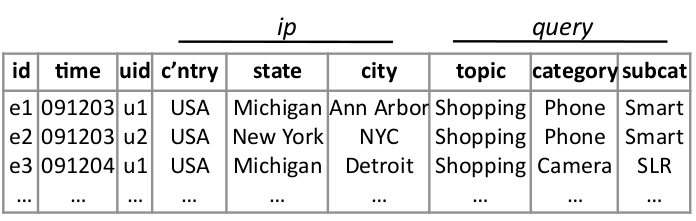
\includegraphics[width=3.5in]{picture/ch_datacube_mr/dataset_table} 
\caption{数据集的表结构}\label{dataset_table} 
\end{figure} 

\begin{figure}[!htb]
\centering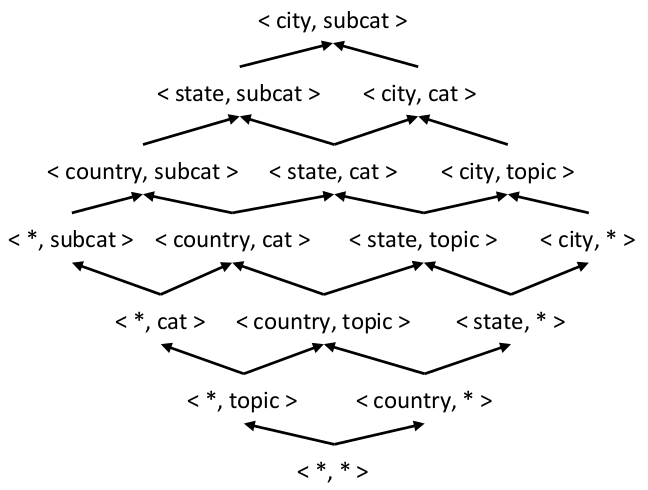
\includegraphics[width=3in]{picture/ch_datacube_mr/dataset_lattice} 
\caption{数据集的lattice}\label{dataset_lattice} 
\end{figure} 

对于该数据集,为了充分比较各种算法的效率与特性,实验中使用了3种不同的数据分布。分别如下:
\begin{itemize}

\item \textbf{D1 分布}

对于属性 country 的取值范围为 [1,3],且是均匀分布的。对于属性 topic 的取值范围为[1,10],且是均匀分布的。剩余的属性取值范围较大,如city取值范围为[1,4000],subcategory 取值范围为[1,20000],且都是均匀分布的。由于country和topic的取值范围较小,因此Region(country)和Region(topic)在数据量较大的数据集中均包含了大的group。

\item \textbf{D2A 分布}

为了出现数据分布更倾斜的情况,即每个region中都有reducer-unfriendly的group,因此该分布中的数据是2/8分的。这里的2/8分指的是该数据集中有80\%的记录,它们之间的6个维属性都是相同的,即它们都属于同一个group,剩下的20\%的数据的分布与 D1 相同。而对于非维属性,它们的取值则无此特性,属性 uid 是均匀分布的。

\item \textbf{D2B 分布}

D2B 的数据分布与 D2A 基本一致,但 uid 是倾斜分布的,若使用求余的方式对数据进行划分,则可能导致划分的不均匀。

\end{itemize}

这三种数据集都有不同程度的倾斜,D1的倾斜度没有D2的明显,并且D1数据集中仅有部分的region是reducer-unfriendly的,例如Region(country)、Region(topic)。而对于D2的数据集,在数据量较大时,每个region都会是reducer-unfriendly的region。对于以上三种分布,属性 uid 的取值范围均为$[1,{10}^{6}]$。由于uid取值范围较大,因此MapReduce的combiner无法充分发挥作用。

实验中分别对代数度量与整体性度量进行比较,代数度量选择 COUNT(*),计算每个group内记录的数量; 整体性度量选择 COUNT(DISTINCT(uid)),计算每个group内不同的uid数量。

数据集中记录的数量分别为${10}^{6}$、${10}^{7}$、${10}^{8}$、${10}^{9}$。对于${10}^{9}$的数据集,大小约为45G。


\section{比较算法}

TSP-Cube 除了与 Naive 和 MR-Cube 的方法比较外,还将与 Naive-PipeSort 与 TopDownCube \cite{lee2012efficient} 进行比较。

Naive-PipeSort 是不对group进行任何划分,只将多个group放在同一个reduce函数内计算,并且使用与TSP-Cube一致的计算方法——PipeSort 计算同一个reduce函数内的多个group。将TSP-Cube与这个方法比较,是为了查看当数据倾斜时,reduce是否会出现严重的负载不均衡,并且查看数据划分是否能提升计算效率。

TopDownCube,是将 PipeSort 与 MapReduce 结合的一种方法。Pipsort最根本的思想是对``数据”不断地排序,这个``数据”可能是原数据,也可能是已经计算好GroupBy的数据。TopDownCube沿用了\cite{agarwal1996computation} 中构造pipe树的方法,并且使用 MapReduce 对每个pipeline中的数据都按照起始 region 的属性顺序进行排序。这个方法的缺点是需要执行多次MapReduce,因为该方法会对于每个 pipeline都执行一次 MapReduce,将数据按照起始region的属性顺序排序。排序后它可以将多个 region 放在同一个 reducer 上计算,并且由于不是所有排序都基于原数据,因此产生的中间数据比 Naive-Pipesort要少。但这种方法并没有考虑整体性度量函数,因此该方法更适合代数度量函数的计算。

实验代码GitHub地址:\url{https://github.com/abcdmyz/MapReduceDataCube}

\section{实验结果}

对以上算法的比较主要包括,在不同的数据分布以及数据大小下,算法的运行时间, 各个reducer输入的记录数。通过算法的运行时间比较各个算法的效率,通过各个 reducer 输入的记录数查看数据划分对各个reducer 之间的负载均衡影响。最后还比较了 MR-Cube 与 TSP-Cube 在第二次MapReduce后,即数据立方计算后,需要合并的数据量和合并过程的运行时间,以及 TSP-Cube 3次MapReduce各占的比例。

以下分别从不同类型的度量函数来分析实验结果。

\subsection{DISTINCT 度量}


图\ref{d1_distinct_time}、 \ref{d2a_distinct_time}、 \ref{d2b_distinct_time} 分别为在 D1, D2A, D2B 三种不同的分布下,5种方法计算COUNT(DISTINCT(uid))度量函数的运行时间。图中的横轴为数据大小,图中的纵轴为运行时间,单位为分钟。从图中可看出,当数据量较小时,5种方法之间的差距并不大,当数据量到达${10}^{9}$时,各种方法之间才有较为明显的差距。图\ref{d1_distinct_input}、图\ref{d2a_distinct_input}、图\ref{d2b_distinct_input} 分别为数据集大小为${10}^{9}$时,各种方法中各个reducer输入的记录数。从这个记录数查看各个reducer之间的负载差距。以下分别分析各种方法的运行时间以及reducer的负载。

\begin{itemize}

\item \textbf{Naive, Naive-PipeSort}

Naive方法 无论在任何一种分布下所花费的时间都是最多的。在D1的数据分布下,Naive-Pipesort的方法的运行时间是最短的,但与MR-Cube和TSP-Cube相比,优势并不大。在D2的分布下,Naive-Pipesort的性能则大打折扣。这是因为对于极端倾斜的数据分布,就算在Naive的基础上加上了PipeSort,但由于D2中的一些group的大小差距非常大(D2是2/8分的分布),而这些大group并没有进行划分,导致 reducer之间的负载极度不均衡,最终仍然使性能下降。由于D2的倾斜性比D1明显,因此Naive-Pipesort的缺点在D2中更能体现。从图\ref{d2a_distinct_input}和图\ref{d2b_distinct_input} 可看出 Naive-PipeSort 的方法各个reducer输入的数据量有较大的差距,尤其有3个reducer输入的数据量特别大,导致了整体的执行时间变长。

\item \textbf{TopDownCube}

对于 TopDownCube的方法,在D1中仅比Naive的方法好,这是因为它要进行多次的MapReduce对数据进行排序,但uid的取值范围较大,无法大量压缩,中间数据仅减少了小部分,多次``低效”的排序导致它需要较长的运行时间。而在D2A分布中,它比Naive-Pipesort的方法有优势。因为 D2A 的数据比 D1 更倾斜,对于Naive-Pipesort而言,其负载不均衡的情况比 TopDownCube更严重。因为TopDown通过对数据多次排序,减少了部分的中间数据,尽管减少的量并不大,但是与Naive-Pipesort相比,能降低负载不均衡的严重性,因此TopDownCube 与 Naive-PipeSort 相比有一定的优势。

但与TSP-Cube相比,在任何一种数据分布中,运行时间都比TSP-Cube的要长,这也是因为数据倾斜导致的。因为TopDown没有对数据进行划分,reducer之间的负载差距依然存在,即使它使用多轮MapReduce减少中间数据。从图\ref{d1_distinct_input}、图\ref{d2a_distinct_input}可看出TopDownCube中各个reducer之间有一定差距,而TPS-Cube的各个reducer之间是非常均匀的。总体而言,将TopDownCube的方法运用在计算整体性度量函数中,优势并不明显。

\item \textbf{MR-Cube, TSP-Cube}

TSP-Cube与MR-Cube相比,在三种分布下,TSP-Cube的运行时间都比MR-Cube少。在D1和D2A中,这种时间优势并不明显,差距并不大,但在D2B中,TSP-Cube的优势则较为明显地体现出来。对于D1,从图\ref{d1_distinct_input} 中可看出,MR-Cube的各个reducer之间要处理的数据量会有一定的差距,而TSP-Cube的各个reducer的数据量非常均匀,因此TSP-Cube比MR-Cube在时间上稍微有优势。

对于D2A,MR-Cube与TSP-Cube的时间差也不大,从图\ref{d2a_distinct_input}中可看出 MR-Cube 与 TSP-Cube 的各个reducer上的数据都是均匀的,导致两者细微的差距是第三轮MapReduce中要合并的数据量的差距。图\ref{d2a_distinct_interdata} 为 MR-Cube与TSP-Cube第三轮需要合并的数据量的比较。从图中可看出,MR-Cube相比TSP-Cube要合并更多的数据,因此需要更多的时间。对于D2B,因为D2B中的uid分布是不均匀的,这样MR-Cube中使用求余的方式对数据进行划分,可能导致划分后的数据依然不均匀。Reducer之间的负载差距则导致MR-Cube性能的下降。在图\ref{d2b_distinct_input}中,由于uid的倾斜性,导致MR-Cube的各个reducer分布不均匀,但TSP-Cube的各个reducer中的数据依然能够均匀分布。因此TSP-Cube比MR-Cube在性能上有较大的优势。

\end{itemize}

\begin{figure}[!ht]
\begin{tabular}{cc}

\begin{minipage}[t]{0.45\textwidth}
\centering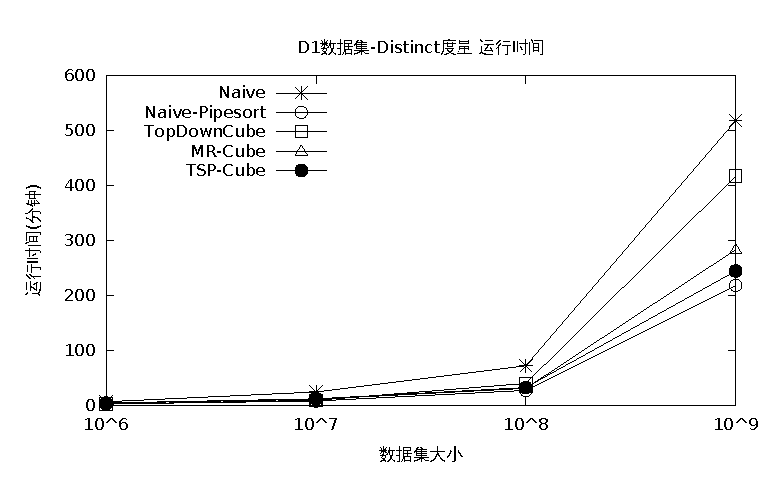
\includegraphics[width=2.7in]{picture/ch_experiment_gnuplot_eps/d1_distinct_time} 
\caption{D1-DISTINCT运行时间}\label{d1_distinct_time} 
\end{minipage}

\begin{minipage}[t]{0.55	\textwidth}
\centering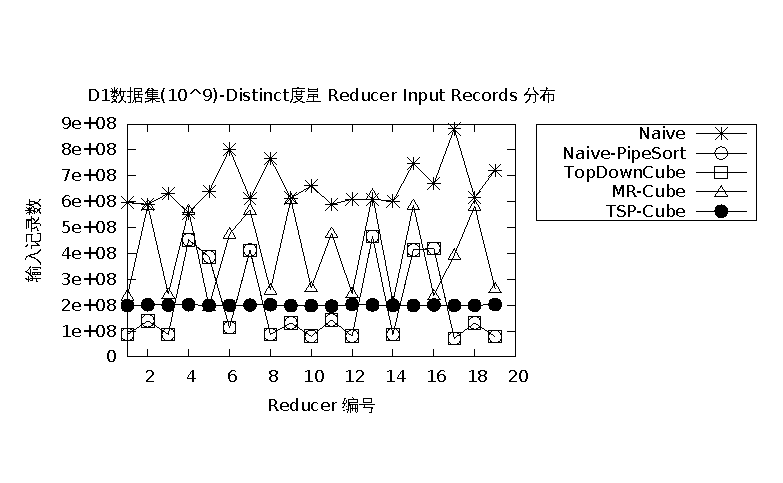
\includegraphics[width=3.2in]{picture/ch_experiment_gnuplot_eps/d1_distinct_input} 
\caption{D1-DISTINCT Reducer Input}\label{d1_distinct_input} 
\end{minipage}

\end{tabular}
\end{figure}



\begin{figure}[!ht]
\begin{tabular}{cc}

\begin{minipage}[t]{0.45\textwidth}
\centering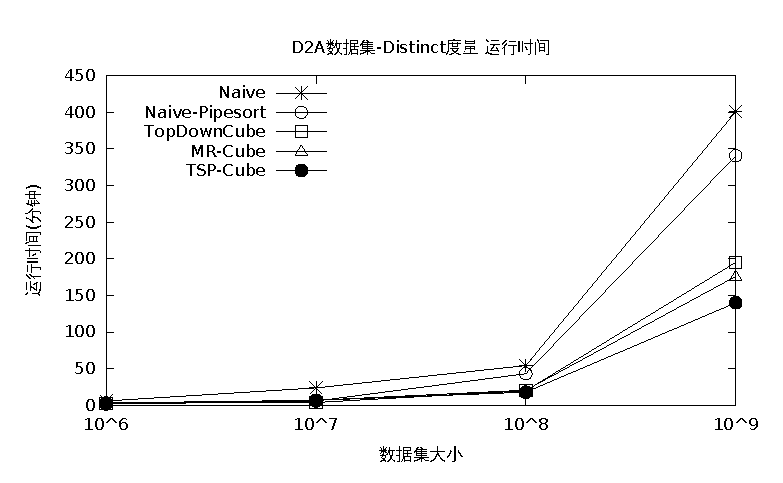
\includegraphics[width=2.7in]{picture/ch_experiment_gnuplot_eps/d2a_distinct_time} 
\caption{D2A-DISTINCT运行时间}\label{d2a_distinct_time} 
\end{minipage}

\begin{minipage}[t]{0.55\textwidth}
\centering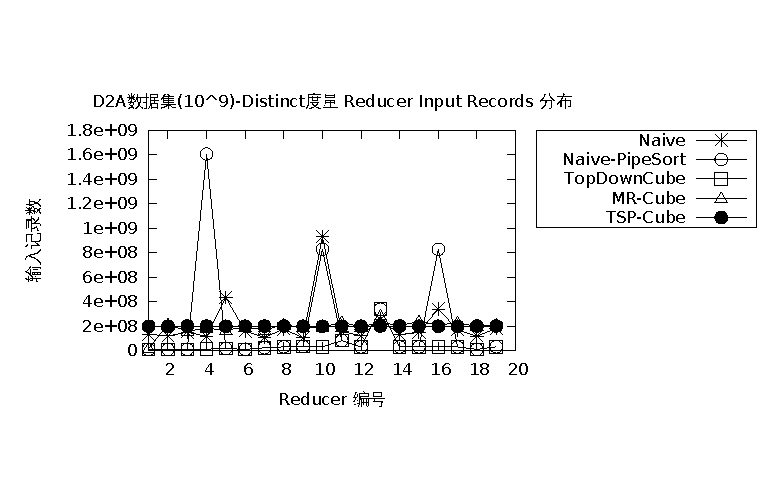
\includegraphics[width=3.2in]{picture/ch_experiment_gnuplot_eps/d2a_distinct_input} 
\caption{D2A-DISTINCT Reducer Input}\label{d2a_distinct_input} 
\end{minipage}

\end{tabular}
\end{figure}


\begin{figure}[!ht]
\begin{tabular}{cc}

\begin{minipage}[t]{0.45\textwidth}
\centering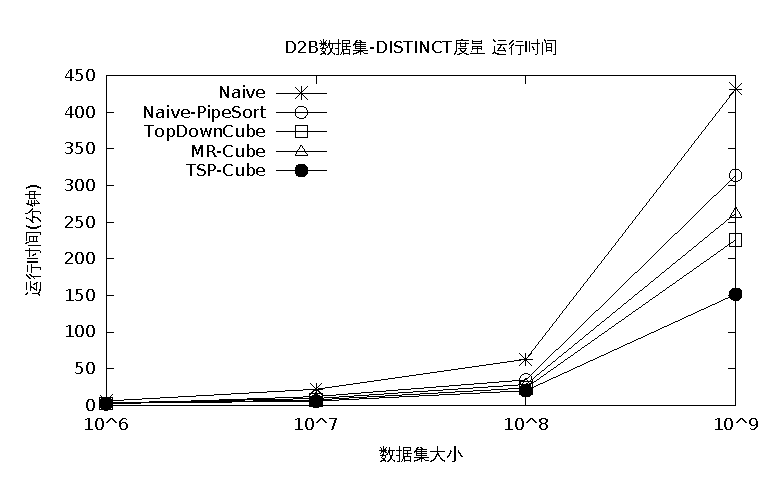
\includegraphics[width=2.7in]{picture/ch_experiment_gnuplot_eps/d2b_distinct_time} 
\caption{D2B-DISTINCT运行时间}\label{d2b_distinct_time} 
\end{minipage}

\begin{minipage}[t]{0.55\textwidth}
\centering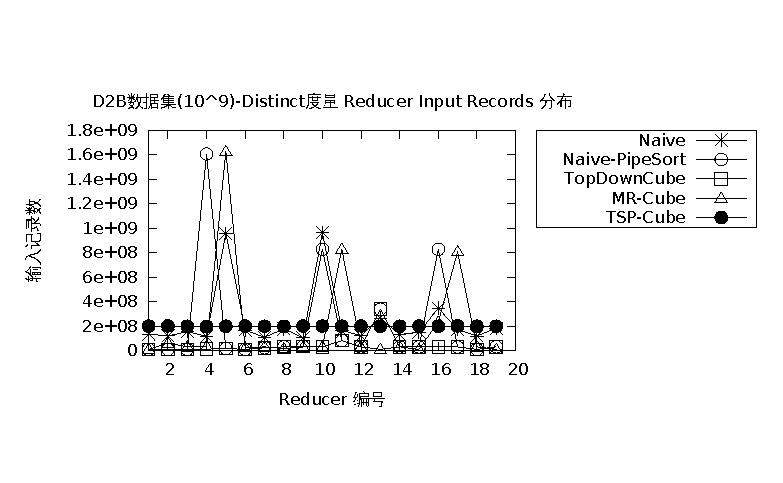
\includegraphics[width=3.2in]{picture/ch_experiment_gnuplot_eps/d2b_distinct_input} 
\caption{D2B-DISTINCT Reducer Input}\label{d2b_distinct_input} 
\end{minipage}

\end{tabular}
\end{figure}


除了比较运行时间与reducer的负载外,以下还将比较MR-Cube与TSP-Cube在不同分布下,在第三轮MapReduce时,需要合并的数据量和合并的运行时间,以及TSP-Cube的3次MapReduce分别占总时间的比例。在前面的章节提到,MR-Cube对group的划分方法在一些场景下会导致不必要的划分,从而加重了之后的合并操作,因此这里将两种方法需要合并的数据量和合并的运行时间进行比较,从而说明TSP-Cube需要进行合并的数据比MR-Cube更少。

图\ref{d1_distinct_interdata}和图\ref{d2a_distinct_interdata}分别为MR-Cube与TSP-Cube在D1和D2A数据分布下,需要合并的数据量。图\ref{d1_distinct_intertime}和图\ref{d2a_distinct_intertime}为合并时间。在D1中,由于数据倾斜性并不明显,因此两者需要合并的数据量差别不大,时间上差别也不大。但在D2A中,由于数据的倾斜性较明显,而MR-Cube会对数据产生不必要的划分,因此随着数据量增大,MR-Cube要合并的数据比TSP-Cube要多,合并时间更长。

图\ref{d1_distinct_mr123}和图\ref{d2a_distinct_mr123} 分别为TSP-Cube在D1和D2A数据分布,数据集大小为 ${10}^{9}$ 下,三次MapReduce占总体时间的比例。随着数据量增大,MR1和MR3所占的比例都会减少。因此花费一定代价对数据进行划分从而使数据分配均匀对总体性能的提升是有意义的。

从以上实验可看出,TSP-Cube相对于其他方法并不是``完美无缺”或者各方面``遥遥领先”的,它在一些数据分布下,跟大部分的方法相比,在性能上的优势并不明显。但在一些较为倾斜的数据分布下,它能表现出它性能的优势。TSP-Cube 无论在一般数据分布下,或者倾斜的数据分布下,均能对数据进行均匀的划分,令各个reducer上的数据负载均衡,从而提升计算性能。并且 TSP-Cube中的PipeSort方法简单且有效,能令数据立方计算过程中的中间数据大大减少,从而也提升了计算性能。因此由以上的实验得出,TSP-Cube 比 MR-Cube 更具有通用性,在一些更为倾斜的数据集下,有明显的优势。





\begin{figure}[!ht]
\begin{tabular}{cc}

\begin{minipage}[t]{0.5\textwidth}
\centering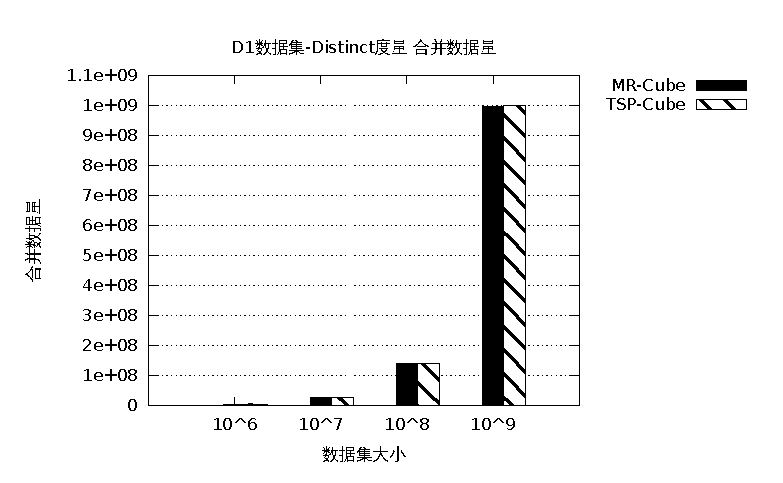
\includegraphics[width=3in]{picture/ch_experiment_gnuplot_eps/d1_distinct_interdata} 
\caption{D1-DISTINCT 合并数据量}\label{d1_distinct_interdata} 
\end{minipage}

\begin{minipage}[t]{0.5\textwidth}
\centering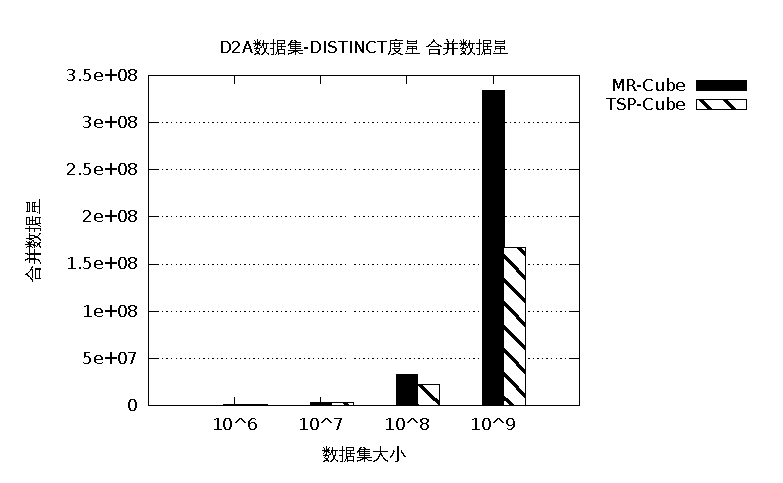
\includegraphics[width=3in]{picture/ch_experiment_gnuplot_eps/d2a_distinct_interdata} 
\caption{D2A-DISTINCT 合并数据量}\label{d2a_distinct_interdata} 
\end{minipage}

\end{tabular}
\end{figure}



\begin{figure}[!ht]
\begin{tabular}{cc}

\begin{minipage}[t]{0.5\textwidth}
\centering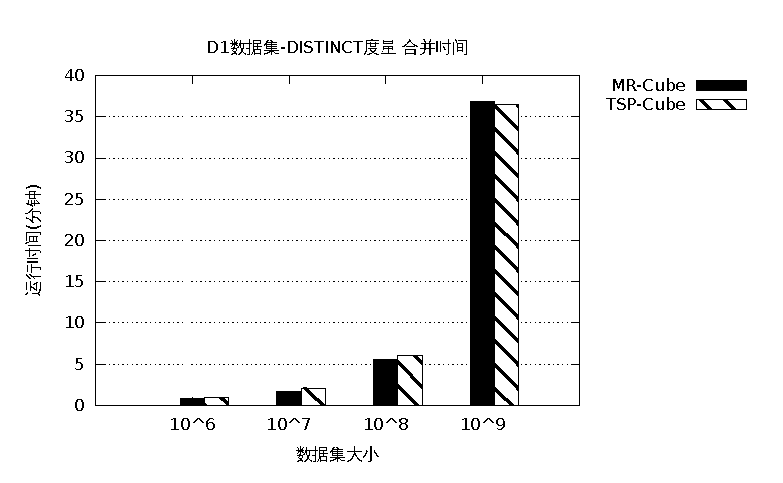
\includegraphics[width=3in]{picture/ch_experiment_gnuplot_eps/d1_distinct_intertime} 
\caption{D1-DISTINCT 合并数据时间}\label{d1_distinct_intertime} 
\end{minipage}

\begin{minipage}[t]{0.5\textwidth}
\centering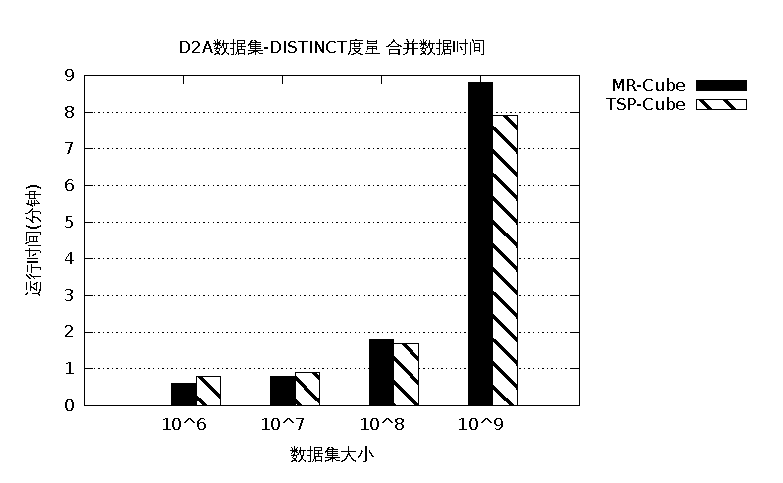
\includegraphics[width=3in]{picture/ch_experiment_gnuplot_eps/d2a_distinct_intertime} 
\caption{D2A-DISTINCT 合并数据时间}\label{d2a_distinct_intertime} 
\end{minipage}

\end{tabular}
\end{figure}





\begin{figure}[!ht]
\begin{tabular}{cc}

\begin{minipage}[t]{0.5\textwidth}
\centering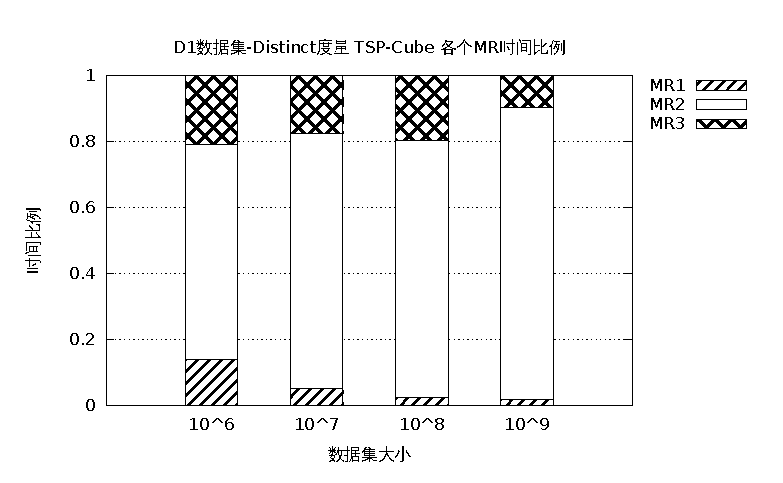
\includegraphics[width=3in]{picture/ch_experiment_gnuplot_eps/d1_distinct_mr123} 
\caption{D1-DISTINCT TSP-Cube 各个MR  运行时间比例}\label{d1_distinct_mr123} 
\end{minipage}

\begin{minipage}[t]{0.5\textwidth}
\centering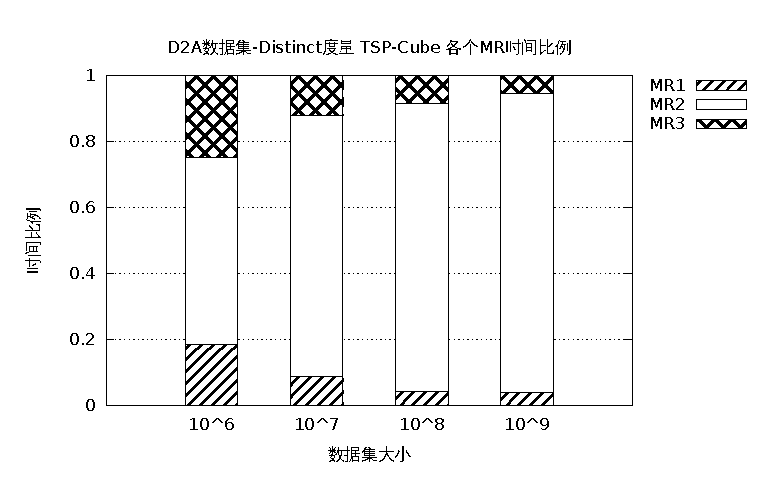
\includegraphics[width=3in]{picture/ch_experiment_gnuplot_eps/d2a_distinct_mr123} 
\caption{D2A-DISTINCT TSP-Cube 各个MR  运行时间比例	}\label{d2a_distinct_mr123} 
\end{minipage}

\end{tabular}
\end{figure}



\subsection{COUNT 度量}

在实验中加入代数度量函数进行对比,从而说明不同类型的度量函数应使用对应合适的方法,在分布式数据立方的计算中,并没有一种万能的方法可以适用于所有的度量函数和所有的场景。以下将5种方法计算COUNT的性能进行比较。图\ref{d1_count_time}、图\ref{d2a_count_time}分别为D1和D2A分布下,5种方法在不同数据大小下的运行时间。图\ref{d1_count_input}、图\ref{d2a_count_input}为不D1和D2A分布下,各个reducer输入的数据量。

从这些图中发现,在DISTINCT度量中性能表现最差的Naive,在COUNT度量中却是性能最好的,无论是在哪种数据分布下。在DISTINCT度量中,由于数据的倾斜性,Naive方法在reducer上数据的分布是非常不均匀的,但是在COUNT度量中,Naive方法在reducer上的数据分布却是非常均匀的,无论在哪种数据分布下。而TSP-Cube和MR-Cube对数据的划分反而导致数据的不均匀。

这个结果的出现与度量函数本身,还有MapReduce框架的特性有非常大的关系。COUNT是代数度量函数,因此数据可以随意划分,并且对于每个分块进行计算的中间结果都是一个整数,或者数据量是固定的。而MapReduce框架有一个非常重要的特性,Combiner。这个Combiner的作用在上一章节中也提到,它等同于本地的reducer。mapper产生的输出并不是直接发给相应的reducer,而是先在本地进行一次reduce计算,再通过网络传输发到reducer上。对于代数度量函数,一个group内的大量数据都可以变成一条数据发到reducer上,因此中间数据大大减少,并且mapper的数量是有限的,那么分发到一个reducer上一个group内的数据也是有限的。这样有限的数据必然不会导致各个reducer上数据的不均匀。

MR-Cube与TSP-Cube的提出,都是为了解决reducer上数据分配不均匀,数据量差别过大的问题,但在代数度量中,这个问题不存在,那么强行使用这两种方法只会带来更差的性能。从图中也可看出,Naive和TopDownCube在性能上比MR-Cube和TSP-Cube更有优势。

Naive-Pipesort的方法在计算COUNT度量时,性能不如Naive的方法,即使Naive-Pipesort方法的中间数据变少了,但性能反而比Naive的差。这是因为Pipesort要求对数据进行排序。MapReduce默认会对key进行排序,但是对于value,若用户不重载相关函数,value是不会排序的。而Pipesort是需要对value进行排序,这里需要花费一定的时间。因此即使Naive的中间数据比Naive-Pipesort多,但因为Naive不需要对value进行排序,因此在性能上能比Naive-Pipesort的更有优势。

\begin{figure}[!ht]
\begin{tabular}{cc}

\begin{minipage}[t]{0.4\textwidth}
\centering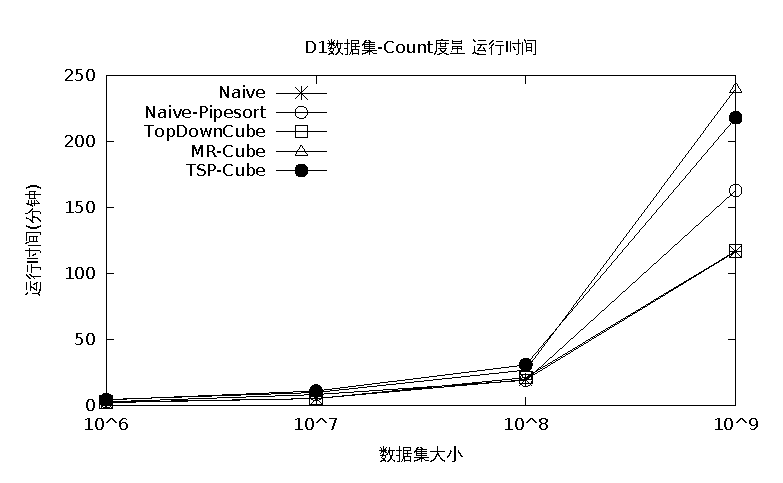
\includegraphics[width=2.7in]{picture/ch_experiment_gnuplot_eps/d1_count_time} 
\caption{D1-COUNT 运行时间}\label{d1_count_time} 
\end{minipage}

\begin{minipage}[t]{0.6\textwidth}
\centering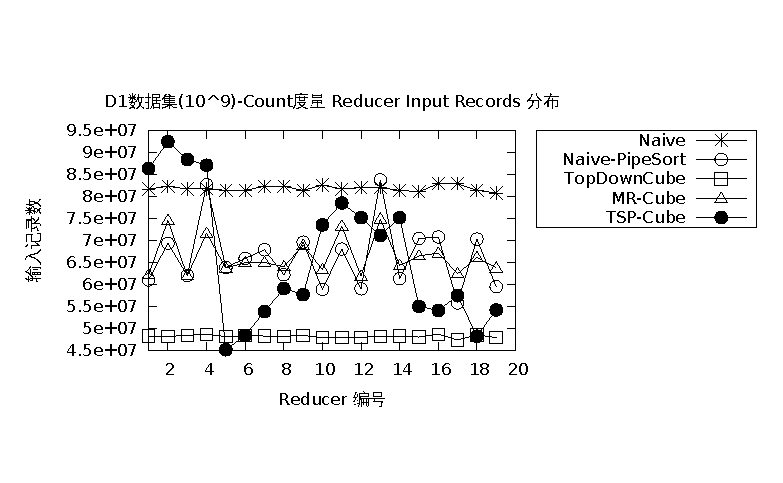
\includegraphics[width=3in]{picture/ch_experiment_gnuplot_eps/d1_count_input} 
\caption{D1-COUNT Reducer Input}\label{d1_count_input} 
\end{minipage}

\end{tabular}
\end{figure}


\begin{figure}[!ht]
\begin{tabular}{cc}

\begin{minipage}[t]{0.4\textwidth}
\centering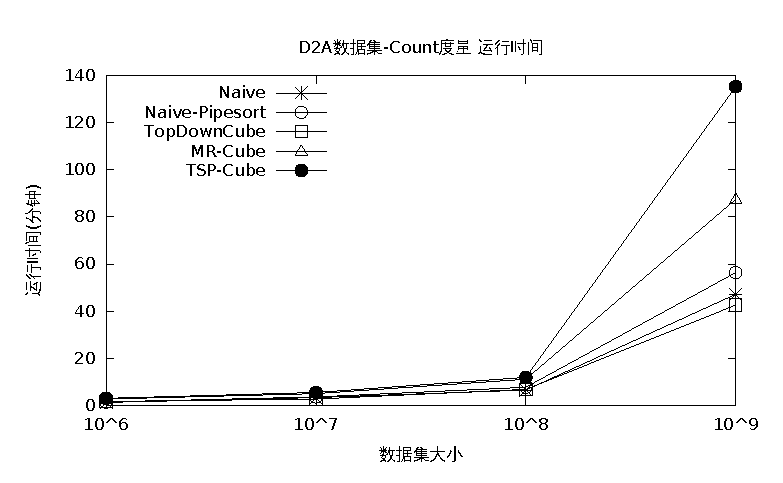
\includegraphics[width=2.7in]{picture/ch_experiment_gnuplot_eps/d2a_count_time} 
\caption{D2A-COUNT 运行时间}\label{d2a_count_time} 
\end{minipage}

\begin{minipage}[t]{0.6\textwidth}
\centering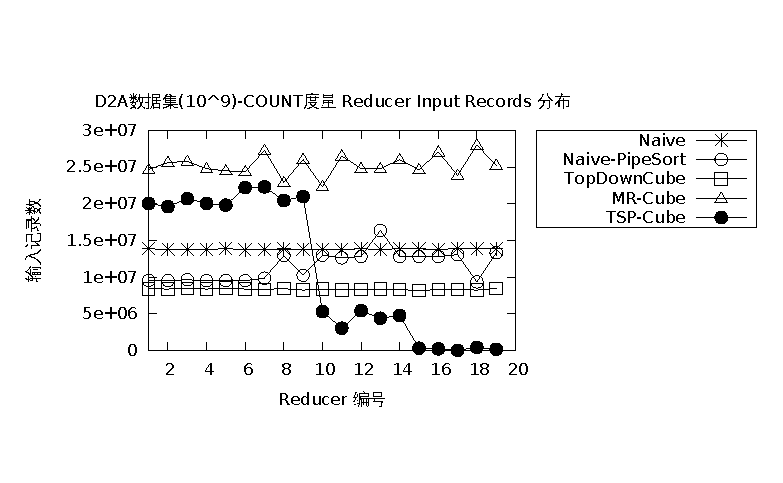
\includegraphics[width=3in]{picture/ch_experiment_gnuplot_eps/d2a_count_input} 
\caption{D2A-COUNT Reducer Input}\label{d2a_count_input} 
\end{minipage}

\end{tabular}
\end{figure}

\section{实验结论}

根据以上的实验,可得知不同的度量函数使用不同的方法会有不同的结果,目前没有一种方法能对于所有的数据分布、所有的度量都适用。在对一种方法进行评估时,需要考虑到它使用的场景(包括度量函数、数据分布等),还需要结合它所基于的框架的特性,来综合评估这种方法。Naive的方法即使简单,也并不是在所有情况下都效率低下,结合框架的特性反而能让它发挥优势。而相对复杂的TSP-Cube方法,则着重于解决一些Naive解决不了的更为极端的情况。

对于代数度量,使用Naive的方法已经足够了。Naive方法实现简单,并且在代数度量中,并不会出现reducer负载不均衡的情况。而对于整体性度量,TSP-Cube与多种算法相比,无论在一般分布或是倾斜分布下,性能都是最好的,尤其在极端倾斜的分布下,其性能优势更为明显。在负载均衡方面,即使在极端倾斜的分布下,TSP-Cube 依然能均匀地划分数据,这也是与其他算法相比最大的优势。由于TSP-Cube 在不同的场景不同的数据分布下,均能保持性能优势,比其他方法更具有通用性,因此建议对于整体性度量函数,使用TSP-Cube的方法。


